\section{Results}
\label{sec:results}

\subsection{The free reference set: OOB versus holdout (H2, H3)}

Table~\ref{tab:main} reports the mean absolute error (MAE) on the 1{,}680 main tasks, and Figure~\ref{fig:bars} visualizes the three variants of each family. Table~\ref{tab:paired} summarizes the planned paired comparisons across all five experiments.

\begin{table}[t]
\centering\small
\caption{Main synthetic benchmark (1{,}680 tasks, $T=200$): MAE in percentage points (mean $\pm$ s.e.) of target-accuracy estimates, by shift type. Bold marks the best estimator in each column. HO: 20\% holdout reference set. OOB: naive OOB plug-in. -X: size-matched extrapolation (ours).}
\label{tab:main}
\begin{tabular}{lccccc}
\toprule
Estimator & IID & Covariate & Corruption & Label & All\\
\midrule
AC & 16.67\,\scriptsize{$\pm$0.44} & 16.02\,\scriptsize{$\pm$0.26} & 13.33\,\scriptsize{$\pm$0.30} & 16.74\,\scriptsize{$\pm$0.47} & 15.45\,\scriptsize{$\pm$0.17} \\
HO & 3.32\,\scriptsize{$\pm$0.22} & 8.08\,\scriptsize{$\pm$0.29} & 11.87\,\scriptsize{$\pm$0.34} & 4.07\,\scriptsize{$\pm$0.24} & 7.91\,\scriptsize{$\pm$0.18} \\
HO\mbox{-}DoC & 3.37\,\scriptsize{$\pm$0.21} & 5.71\,\scriptsize{$\pm$0.20} & 6.07\,\scriptsize{$\pm$0.25} & 3.82\,\scriptsize{$\pm$0.22} & 5.21\,\scriptsize{$\pm$0.12} \\
HO\mbox{-}ATC & 4.08\,\scriptsize{$\pm$0.26} & 8.33\,\scriptsize{$\pm$0.28} & 9.01\,\scriptsize{$\pm$0.35} & 4.48\,\scriptsize{$\pm$0.28} & 7.37\,\scriptsize{$\pm$0.17} \\
HO\mbox{-}IW & 5.82\,\scriptsize{$\pm$0.41} & 9.96\,\scriptsize{$\pm$0.35} & 13.28\,\scriptsize{$\pm$0.40} & 6.91\,\scriptsize{$\pm$0.44} & 9.88\,\scriptsize{$\pm$0.22} \\
OOB & 1.91\,\scriptsize{$\pm$0.12} & 6.02\,\scriptsize{$\pm$0.25} & 10.69\,\scriptsize{$\pm$0.32} & 2.76\,\scriptsize{$\pm$0.18} & 6.30\,\scriptsize{$\pm$0.16} \\
OOB\mbox{-}DoC & 1.99\,\scriptsize{$\pm$0.12} & 4.52\,\scriptsize{$\pm$0.15} & \textbf{4.24\,\scriptsize{$\pm$0.17}} & 2.70\,\scriptsize{$\pm$0.17} & \textbf{3.82\,\scriptsize{$\pm$0.09}} \\
OOB\mbox{-}ATC & 2.66\,\scriptsize{$\pm$0.18} & 7.45\,\scriptsize{$\pm$0.24} & 7.94\,\scriptsize{$\pm$0.30} & 3.17\,\scriptsize{$\pm$0.20} & 6.29\,\scriptsize{$\pm$0.15} \\
OOB\mbox{-}IW & 2.42\,\scriptsize{$\pm$0.17} & 4.71\,\scriptsize{$\pm$0.18} & 10.72\,\scriptsize{$\pm$0.33} & 2.92\,\scriptsize{$\pm$0.19} & 5.84\,\scriptsize{$\pm$0.15} \\
OOB\mbox{-}X & 1.80\,\scriptsize{$\pm$0.12} & 6.38\,\scriptsize{$\pm$0.25} & 11.19\,\scriptsize{$\pm$0.32} & 2.63\,\scriptsize{$\pm$0.17} & 6.56\,\scriptsize{$\pm$0.17} \\
OOB\mbox{-}DoC\mbox{-}X & \textbf{1.74\,\scriptsize{$\pm$0.11}} & \textbf{4.48\,\scriptsize{$\pm$0.15}} & 4.64\,\scriptsize{$\pm$0.19} & \textbf{2.45\,\scriptsize{$\pm$0.15}} & 3.84\,\scriptsize{$\pm$0.09} \\
OOB\mbox{-}ATC\mbox{-}X & 2.11\,\scriptsize{$\pm$0.13} & 6.47\,\scriptsize{$\pm$0.22} & 6.71\,\scriptsize{$\pm$0.28} & 2.48\,\scriptsize{$\pm$0.15} & 5.34\,\scriptsize{$\pm$0.13} \\
OOB\mbox{-}IW\mbox{-}X & 2.24\,\scriptsize{$\pm$0.16} & 4.61\,\scriptsize{$\pm$0.18} & 11.16\,\scriptsize{$\pm$0.34} & 2.79\,\scriptsize{$\pm$0.18} & 5.88\,\scriptsize{$\pm$0.15} \\
\bottomrule
\end{tabular}
\end{table}

\begin{figure}[t]
\centering
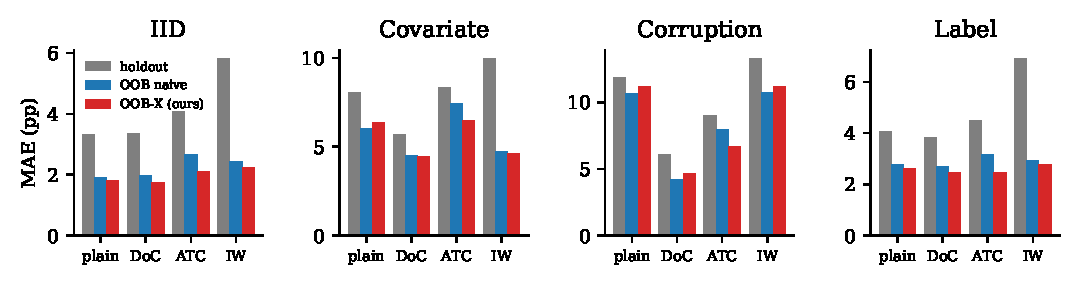
\includegraphics[width=\linewidth]{figs/main_bars.pdf}
\caption{MAE by estimator family and shift type on the main benchmark. In every panel and every family, both OOB routes (blue, red) improve on the holdout route (grey).}
\label{fig:bars}
\end{figure}

\begin{table}[t]
\centering\small
\caption{Planned paired comparisons of holdout (HO-$\Phi$) against size-extrapolated OOB (OOB-$\Phi$-X) estimators in all six experiments. $\Delta$: relative MAE reduction. Win: fraction of tasks in which OOB-X has lower absolute error. All 24 comparisons are significant after Holm correction within each experiment (two-sided Wilcoxon signed-rank test; the largest adjusted $p$ is $0.045$, for DoC on the small real datasets; all others are $<10^{-3}$).}
\label{tab:paired}
\begin{tabular}{lrcccccccc}
\toprule
 & & \multicolumn{2}{c}{plain} & \multicolumn{2}{c}{DoC} & \multicolumn{2}{c}{ATC} & \multicolumn{2}{c}{IW}\\
\cmidrule(lr){3-4}\cmidrule(lr){5-6}\cmidrule(lr){7-8}\cmidrule(lr){9-10}
Experiment & tasks & $\Delta$ & win & $\Delta$ & win & $\Delta$ & win & $\Delta$ & win\\
\midrule
Main (synthetic) & 1680 & 17\% & .64 & 26\% & .63 & 27\% & .65 & 40\% & .72\\
Ensemble-size sweep & 600 & 9\% & .57 & 14\% & .58 & 25\% & .64 & 22\% & .66\\
Sample-size sweep & 720 & 11\% & .64 & 23\% & .62 & 26\% & .63 & 29\% & .72\\
Real datasets (small) & 420 & 17\% & .63 & 7\% & .55 & 39\% & .67 & 33\% & .68\\
OpenML-CC18 (72 datasets) & 1512 & 6\% & .59 & 5\% & .55 & 11\% & .61 & 21\% & .67\\
Extra-Trees & 280 & 10\% & .65 & 14\% & .63 & 13\% & .64 & 26\% & .68\\
\bottomrule
\end{tabular}
\end{table}

\paragraph{H2 is supported in every comparison.}
Across six experiments, four estimator families and 5{,}212 tasks, the OOB route beats the holdout route in all 24 planned comparisons, with relative MAE reductions of 5--40\%. Reductions are smaller on the 72 real OpenML datasets (5--21\%) than on synthetic data (Section~\ref{sec:openml}). The gain is largest for importance weighting (21--40\%), as the variance argument in Section~\ref{sec:method} predicts: density-ratio weights shrink the effective size of an already small holdout set. The overall best estimator on the main benchmark is OOB-DoC-X (Friedman average rank 4.85 of 13; Friedman $p<10^{-100}$), followed by naive OOB-DoC (5.11) and OOB-ATC-X (5.94). The best holdout estimator, HO-DoC, ranks fourth (6.29). OOB-DoC-X is within 2\,pp of the true accuracy in 39\% of tasks and within 5\,pp in 73\%. For HO-DoC the figures are 31\% and 62\%.

\paragraph{The advantage is largest with little data.}
At $n=200$ the OOB route reduces MAE by 33\% (DoC), 38\% (ATC) and 50\% (IW; 12.9 vs.\ 6.5\,pp). At $n=1000$ the reductions are 13\%, 12\% and 23\% (all $p<10^{-9}$). The sample-size sweep (Figure~\ref{fig:nsweep}) shows the same pattern: at $n=100$ the IW error drops from 14.1 to 8.4\,pp and the ATC error from 11.9 to 6.7\,pp, and the two routes converge by $n\approx3200$, where a 20\% holdout already holds 640 points.

\begin{figure}[t]
\centering
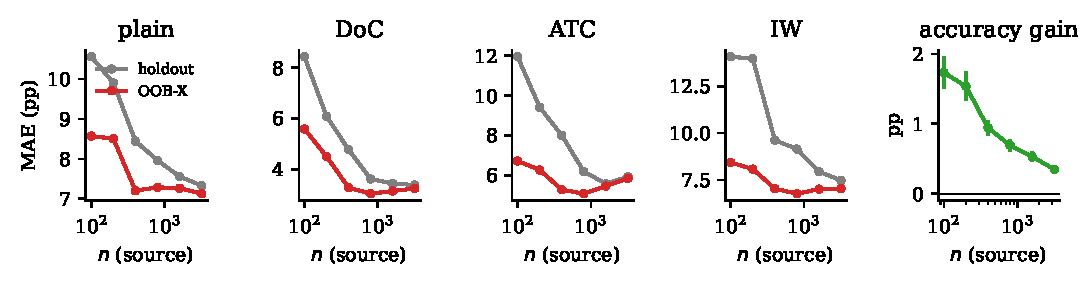
\includegraphics[width=\linewidth]{figs/nsweep.pdf}
\caption{Sample-size sweep (720 tasks; IID, covariate and corruption shift pooled). Left four panels: MAE of holdout versus OOB-X estimators. Right: target-accuracy gain of the model trained on all source data over the model trained on 80\% of it (mean $\pm$ s.e.).}
\label{fig:nsweep}
\end{figure}

\paragraph{H3 is supported: no accuracy tax.}
Because the OOB route needs no holdout, the deployed forest trains on 25\% more data. Its target accuracy is higher by 1.21\,pp on average on the main benchmark (better in 82\% of tasks, $p<10^{-170}$), by 0.96\,pp in the sample-size sweep, by 0.65\,pp for Extra-Trees and by 0.50\,pp on the real datasets. The gain decays smoothly with $n$, from 1.73\,pp at $n=100$ to 0.35\,pp at $n=3200$ (Figure~\ref{fig:nsweep}, right). The OOB route is therefore better on \emph{both} axes of the dilemma described in the introduction: a better model, and a better estimate of how good it is.

\subsection{The size mismatch and size-matched extrapolation (H1)}
\label{sec:mech}

\paragraph{Proposition~\ref{prop:oob} holds empirically.}
Figure~\ref{fig:mech}(a) compares, for 12 synthetic tasks with $T=500$, the OOB accuracy of size-$m$ sub-ensembles with the true target accuracy of size-$m$ ensembles. In-distribution, the gap is statistically indistinguishable from zero at every $m$ from 1 to 160 (means between $-0.37$ and $-0.01$\,pp, each within about one standard error). Once sizes are matched, the OOB sample is an unbiased reference sample, exactly as Proposition~\ref{prop:oob} states. Under covariate shift the gap is 2.7--7.0\,pp; this is the shift-induced change that shift-aware estimators must correct.

\paragraph{The $1/m$ law holds.}
Over the window $m\in[8,60]$, the fit $a+b/m$ explains the target-accuracy curve with median $R^2=0.992$ (IID) and $0.991$ (covariate); 96\% of the target-curve fits have $R^2>0.9$. Extrapolating from $m\le160$ to $T=500$ reduces the error with respect to the true full-ensemble accuracy from 0.54 to 0.28\,pp (Figure~\ref{fig:mech}(b,c)).

\begin{figure}[t]
\centering
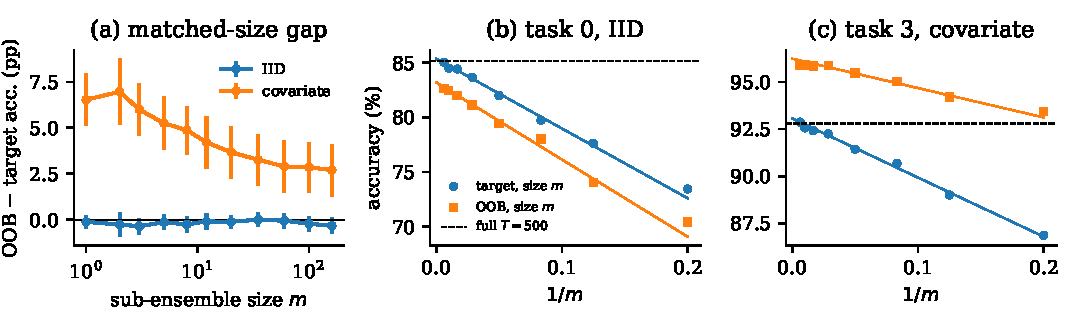
\includegraphics[width=\linewidth]{figs/mech.pdf}
\caption{Mechanism. (a) OOB accuracy minus target accuracy at matched sub-ensemble size $m$, averaged over 12 tasks (mean $\pm$ s.e.). In-distribution the gap is zero at every size (Proposition~\ref{prop:oob}). (b, c) Accuracy against $1/m$ with $a+b/m$ fits on $m\in[8,60]$. The intercept approximates the full ensemble (dashed line).}
\label{fig:mech}
\end{figure}

\paragraph{Naive OOB bias scales as $1/T$; extrapolation removes most of it.}
Figure~\ref{fig:tsweep} (top) shows the in-distribution bias as a function of $T$. The naive plug-ins are biased downwards, and the bias halves each time $T$ doubles. For the plain estimator it is $-3.98$, $-2.19$, $-1.19$, $-0.68$ and $-0.34$\,pp at $T=25,\dots,500$, as Proposition~\ref{prop:bias}(i) predicts. Size-matched extrapolation removes roughly 40--95\% of this bias. For DoC it goes from $-5.77$ to $-2.16$\,pp at $T=25$ and from $-1.50$ to $-0.19$\,pp at $T=100$; for ATC, from $-1.21$ to $-0.16$\,pp at $T=100$. The holdout estimators carry no size bias but have 1.6--3$\times$ the in-distribution MAE of the OOB-X estimators at every $T\ge100$.

\begin{figure}[t]
\centering
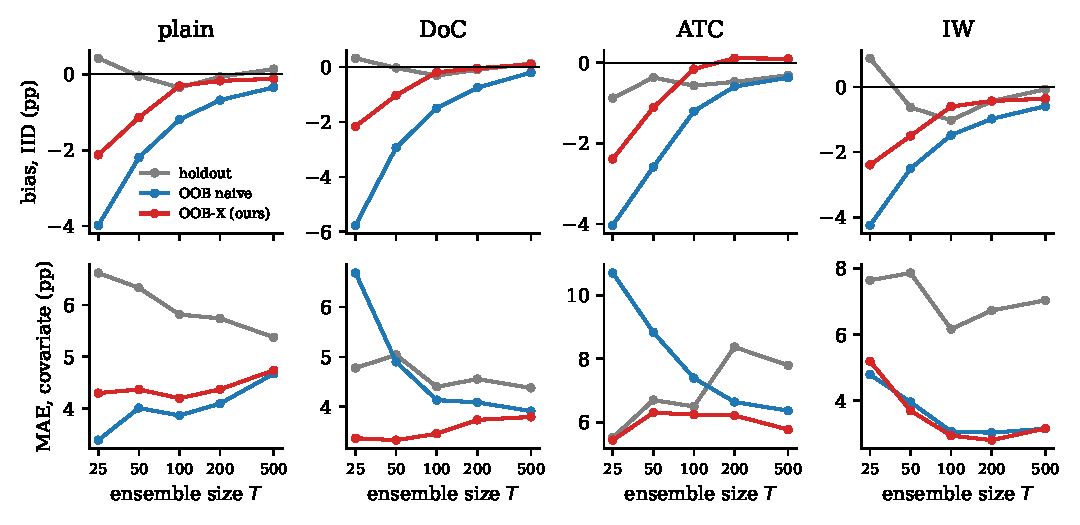
\includegraphics[width=\linewidth]{figs/tsweep.pdf}
\caption{Ensemble-size sweep (600 tasks, $n=500$). Top: signed bias in-distribution; the naive OOB bias decays as $1/T$, and extrapolation removes most of it. Bottom: MAE under covariate shift ($\alpha=2$).}
\label{fig:tsweep}
\end{figure}

\paragraph{When does extrapolation help under shift? A refinement of H1.}
Removing the size bias does not always reduce the error under shift, because the size bias can partly cancel a shift bias of the opposite sign. The outcome is consistent across experiments (Table~\ref{tab:x}).
\emph{ATC}: extrapolation reduces MAE in all six experiments (by 5--29\%, all Holm-adjusted $p<10^{-3}$). Its gains are largest under covariate shift and for small $T$; at $T=25$ under covariate shift the MAE falls from 10.7 to 5.4\,pp.
\emph{DoC}: the effect is neutral to slightly positive (MAE changes between $-4.7\%$ and $+2.1\%$; significant improvements on both real-data experiments, Extra-Trees and the ensemble-size sweep).
\emph{Plain and IW}: extrapolation removes their in-distribution bias but changes MAE by $-0.1\%$ to $+4.7\%$, because under shift these estimators already \emph{over}-estimate accuracy, and correcting the size bias moves them further upward.
We therefore recommend the extrapolated variants for ATC and DoC by default, and the extrapolated plain and IW variants only when the shift is believed to be small.

\begin{table}[t]
\centering\small
\caption{Effect of size-matched extrapolation: relative MAE change of OOB-$\Phi$-X versus naive OOB-$\Phi$ (negative values are improvements). $^{*}$: Holm-adjusted $p<0.01$ (Wilcoxon).}
\label{tab:x}
\begin{tabular}{lcccc}
\toprule
Experiment & plain & DoC & ATC & IW\\
\midrule
Main & $+4.1\%^{*}$ & $+0.7\%$ & $-15.1\%^{*}$ & $+0.7\%^{*}$\\
Ensemble-size sweep & $+4.7\%^{*}$ & $-4.5\%^{*}$ & $-29.3\%^{*}$ & $+2.9\%^{*}$\\
Sample-size sweep & $+3.3\%^{*}$ & $+2.1\%$ & $-9.5\%^{*}$ & $+1.3\%^{*}$\\
Real datasets (small) & $+2.5\%^{*}$ & $-3.0\%^{*}$ & $-7.8\%^{*}$ & $-0.0\%$\\
OpenML-CC18 & $+1.5\%^{*}$ & $-1.6\%^{*}$ & $-5.3\%^{*}$ & $+0.6\%^{*}$\\
Extra-Trees & $+4.2\%^{*}$ & $-4.7\%^{*}$ & $-13.6\%^{*}$ & $-0.1\%$\\
\bottomrule
\end{tabular}
\end{table}

\subsection{Large-scale real-data validation: OpenML-CC18}
\label{sec:openml}

The synthetic results could reflect the generator rather than real tabular data, so we repeated the full protocol on all 72 datasets of OpenML-CC18 (1{,}512 tasks; Table~\ref{tab:openml}, Figure~\ref{fig:openml}). This experiment was run after all others, and the analysis was fixed in advance.

\paragraph{The free reference set replicates, with smaller effects.}
At the task level the OOB route again beats the holdout route in all four families (Table~\ref{tab:paired}), but with smaller relative MAE reductions than on synthetic data: 6\% (plain), 5\% (DoC), 11\% (ATC) and 21\% (IW). At the more conservative \emph{dataset} level (72 paired dataset means), all four improvements remain significant after Holm correction ($p_{\mathrm{Holm}}=0.008$ for DoC, $<10^{-4}$ for the others). OOB-X is better on 54/72 datasets (plain), 45/72 (DoC), 53/72 (ATC) and 66/72 (IW). The deployed model is again more accurate, by 0.59\,pp on average, and better on 59 of the 72 datasets ($p<10^{-9}$).

\paragraph{Where the gain comes from.}
The benefit depends strongly on the shift type. It is largest in-distribution (30--47\% lower MAE in every family) and under sub-population covariate shift (9--42\%; IW falls from 5.96 to 3.48\,pp), moderate under label shift (7--17\%), and close to zero under corruption. There, plain and DoC show no significant difference ($p_{\mathrm{Holm}}=1.0$) and ATC and IW improve by only 6\%. This is expected: once corruption moves the target outside the source support, the error is dominated by the estimator's modelling assumption rather than by reference-set variance, and a larger reference set cannot fix the wrong assumption. The gain also shrinks with dataset size. For datasets with source size $n<700$, MAE falls by 12--25\%; for datasets at the 2{,}000-point cap, by 2--15\%. The improvement for DoC is not significant on medium and large datasets ($p=0.10$ and $0.06$).

\paragraph{Extrapolation.}
The pattern of Table~\ref{tab:x} replicates: extrapolation improves ATC (5.3\% lower MAE, better on 56/72 datasets) and DoC (1.6\%, 45/72), and slightly worsens plain (1.5\%) and IW (0.6\%) estimators.

\paragraph{Shift-type ranking on real data.}
OOB-IW-X is the best estimator under covariate shift (3.48\,pp) and OOB-DoC-X under corruption (10.44\,pp), while ATC fails badly under real-data corruption (at least 18.9\,pp in every variant): its threshold transfers poorly when confidences collapse. The best overall Friedman ranks belong to OOB-IW (5.80), OOB-DoC-X and OOB-IW-X (both 5.82), against 6.41 for the best holdout estimator (HO-DoC).

\begin{table}[t]
\centering\small
\caption{OpenML-CC18 (72 real datasets, 1{,}512 tasks, $T=200$): MAE in pp (mean $\pm$ s.e.).}
\label{tab:openml}
\begin{tabular}{lccccc}
\toprule
Estimator & IID & Covariate & Corruption & Label & All\\
\midrule
AC & 9.62\,\scriptsize{$\pm$0.68} & 11.02\,\scriptsize{$\pm$0.40} & 15.45\,\scriptsize{$\pm$0.64} & 12.21\,\scriptsize{$\pm$0.73} & 12.26\,\scriptsize{$\pm$0.29} \\
HO & 2.04\,\scriptsize{$\pm$0.15} & 6.96\,\scriptsize{$\pm$0.26} & 12.70\,\scriptsize{$\pm$0.59} & 6.41\,\scriptsize{$\pm$0.64} & 7.82\,\scriptsize{$\pm$0.24} \\
HO\mbox{-}DoC & 1.83\,\scriptsize{$\pm$0.14} & 4.19\,\scriptsize{$\pm$0.16} & 10.52\,\scriptsize{$\pm$0.40} & 4.92\,\scriptsize{$\pm$0.50} & 5.77\,\scriptsize{$\pm$0.17} \\
HO\mbox{-}ATC & 2.48\,\scriptsize{$\pm$0.17} & 5.96\,\scriptsize{$\pm$0.27} & 20.14\,\scriptsize{$\pm$0.86} & 4.40\,\scriptsize{$\pm$0.38} & 9.29\,\scriptsize{$\pm$0.33} \\
HO\mbox{-}IW & 2.61\,\scriptsize{$\pm$0.20} & 5.96\,\scriptsize{$\pm$0.25} & 13.86\,\scriptsize{$\pm$0.59} & 6.04\,\scriptsize{$\pm$0.56} & 7.75\,\scriptsize{$\pm$0.24} \\
OOB & 1.37\,\scriptsize{$\pm$0.10} & 6.10\,\scriptsize{$\pm$0.24} & 12.43\,\scriptsize{$\pm$0.60} & 5.93\,\scriptsize{$\pm$0.63} & 7.21\,\scriptsize{$\pm$0.24} \\
OOB\mbox{-}DoC & 1.38\,\scriptsize{$\pm$0.11} & 3.96\,\scriptsize{$\pm$0.15} & 10.48\,\scriptsize{$\pm$0.40} & 4.59\,\scriptsize{$\pm$0.50} & 5.55\,\scriptsize{$\pm$0.17} \\
OOB\mbox{-}ATC & 2.01\,\scriptsize{$\pm$0.15} & 5.11\,\scriptsize{$\pm$0.22} & 19.68\,\scriptsize{$\pm$0.81} & 4.10\,\scriptsize{$\pm$0.42} & 8.69\,\scriptsize{$\pm$0.32} \\
OOB\mbox{-}IW & 1.47\,\scriptsize{$\pm$0.12} & 3.52\,\scriptsize{$\pm$0.17} & 12.79\,\scriptsize{$\pm$0.57} & 5.00\,\scriptsize{$\pm$0.52} & 6.09\,\scriptsize{$\pm$0.22} \\
OOB\mbox{-}X & 1.30\,\scriptsize{$\pm$0.10} & 6.22\,\scriptsize{$\pm$0.24} & 12.68\,\scriptsize{$\pm$0.60} & 5.93\,\scriptsize{$\pm$0.63} & 7.32\,\scriptsize{$\pm$0.24} \\
OOB\mbox{-}DoC\mbox{-}X & \textbf{1.27\,\scriptsize{$\pm$0.09}} & 3.84\,\scriptsize{$\pm$0.15} & \textbf{10.44\,\scriptsize{$\pm$0.40}} & 4.53\,\scriptsize{$\pm$0.50} & \textbf{5.46\,\scriptsize{$\pm$0.17}} \\
OOB\mbox{-}ATC\mbox{-}X & 1.65\,\scriptsize{$\pm$0.12} & 4.77\,\scriptsize{$\pm$0.21} & 18.90\,\scriptsize{$\pm$0.80} & \textbf{3.86\,\scriptsize{$\pm$0.42}} & 8.23\,\scriptsize{$\pm$0.31} \\
OOB\mbox{-}IW\mbox{-}X & 1.37\,\scriptsize{$\pm$0.10} & \textbf{3.48\,\scriptsize{$\pm$0.17}} & 13.02\,\scriptsize{$\pm$0.57} & 5.01\,\scriptsize{$\pm$0.52} & 6.12\,\scriptsize{$\pm$0.23} \\
\bottomrule
\end{tabular}
\end{table}

\begin{figure}[t]
\centering
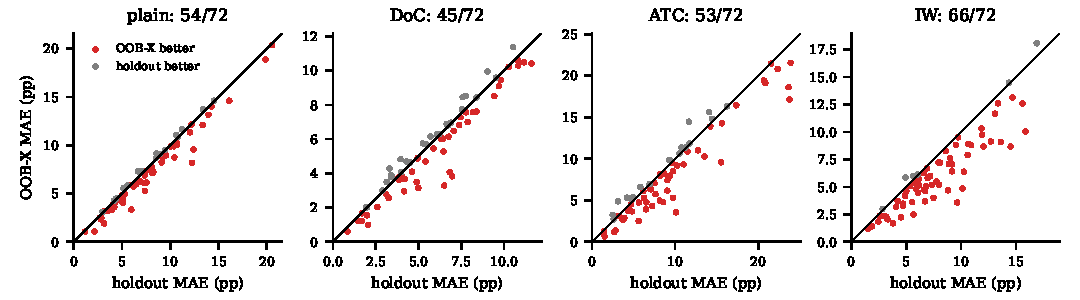
\includegraphics[width=\linewidth]{figs/openml_scatter.pdf}
\caption{OpenML-CC18, one point per dataset: mean absolute error of the holdout estimator (x) against the size-extrapolated OOB estimator (y). Points below the diagonal (red) are datasets where the free reference set is better; titles give the count out of 72.}
\label{fig:openml}
\end{figure}

\subsection{Shift-type dependence (H4)}

H4 is only \emph{partly} supported. Under corruption, which is a support shift, confidence-based estimators dominate on synthetic data, as hypothesized: OOB-DoC reaches 4.2\,pp while every IW variant is at or above 10.7\,pp, because importance weighting cannot extrapolate beyond the source support. Under sub-population covariate shift, however, IW does \emph{not} dominate on synthetic data: OOB-IW-X (4.61\,pp) and OOB-DoC-X (4.48\,pp) are statistically tied. On the three small real datasets the ordering changes: IW and plain OOB are best overall (OOB-IW-X 4.46\,pp), ATC-X is best under covariate shift (3.79\,pp), and every method fails under the strong real-data corruption (all $\ge7.8$\,pp). Label shift of the strength we used produced small accuracy changes, and all OOB-X estimators stayed within 2.8\,pp on average. In short, no estimator family is uniformly best. On synthetic data the benefit of the free reference set holds within every family and every shift type (Figure~\ref{fig:bars}); on OpenML it holds in every family but disappears for plain and DoC estimators under corruption (Section~\ref{sec:openml}).

\subsection{Small real datasets and Extra-Trees (H5)}

On the three small scikit-learn datasets (Table~\ref{tab:real}) the best estimator is an OOB variant in every column, and OOB-IW-X attains the lowest overall MAE (4.46\,pp, versus 5.59\,pp for the best holdout estimator). Per dataset, the best OOB-X estimator improves on the best holdout estimator for Breast Cancer (2.38 vs.\ 3.30\,pp), Digits (4.78 vs.\ 6.31) and Wine (4.18 vs.\ 5.75).
For bootstrapped Extra-Trees \citep{geurts2006et}, all four OOB-X estimators again beat their holdout counterparts (10--26\% lower MAE, all Holm $p<10^{-3}$; Table~\ref{tab:paired}), and the extrapolation pattern of Table~\ref{tab:x} repeats. H5 is supported.

\begin{table}[t]
\centering\small
\caption{Real datasets (Breast Cancer, Digits, Wine; 420 tasks, $T=200$): MAE in pp (mean $\pm$ s.e.).}
\label{tab:real}
\begin{tabular}{lccccc}
\toprule
Estimator & IID & Covariate & Corruption & Label & All\\
\midrule
AC & 12.06\,\scriptsize{$\pm$1.12} & 16.23\,\scriptsize{$\pm$0.72} & 22.56\,\scriptsize{$\pm$1.30} & 12.29\,\scriptsize{$\pm$1.07} & 16.88\,\scriptsize{$\pm$0.56} \\
HO & 2.82\,\scriptsize{$\pm$0.37} & 5.35\,\scriptsize{$\pm$0.43} & 8.88\,\scriptsize{$\pm$0.61} & 2.47\,\scriptsize{$\pm$0.26} & 5.59\,\scriptsize{$\pm$0.28} \\
HO\mbox{-}DoC & 2.87\,\scriptsize{$\pm$0.41} & 6.03\,\scriptsize{$\pm$0.34} & 10.56\,\scriptsize{$\pm$0.55} & 2.15\,\scriptsize{$\pm$0.24} & 6.32\,\scriptsize{$\pm$0.27} \\
HO\mbox{-}ATC & 3.05\,\scriptsize{$\pm$0.55} & 7.38\,\scriptsize{$\pm$0.75} & 14.75\,\scriptsize{$\pm$1.05} & 3.04\,\scriptsize{$\pm$0.51} & 8.25\,\scriptsize{$\pm$0.50} \\
HO\mbox{-}IW & 2.82\,\scriptsize{$\pm$0.43} & 7.57\,\scriptsize{$\pm$0.82} & 9.37\,\scriptsize{$\pm$0.64} & 2.42\,\scriptsize{$\pm$0.28} & 6.67\,\scriptsize{$\pm$0.42} \\
OOB & 1.47\,\scriptsize{$\pm$0.17} & 3.89\,\scriptsize{$\pm$0.39} & 8.52\,\scriptsize{$\pm$0.62} & 1.45\,\scriptsize{$\pm$0.14} & 4.52\,\scriptsize{$\pm$0.28} \\
OOB\mbox{-}DoC & 1.47\,\scriptsize{$\pm$0.16} & 5.79\,\scriptsize{$\pm$0.29} & 10.99\,\scriptsize{$\pm$0.62} & 1.59\,\scriptsize{$\pm$0.14} & 6.06\,\scriptsize{$\pm$0.28} \\
OOB\mbox{-}ATC & 1.52\,\scriptsize{$\pm$0.19} & 4.19\,\scriptsize{$\pm$0.42} & 11.39\,\scriptsize{$\pm$0.81} & 1.60\,\scriptsize{$\pm$0.21} & 5.50\,\scriptsize{$\pm$0.35} \\
OOB\mbox{-}IW & 1.51\,\scriptsize{$\pm$0.19} & 4.28\,\scriptsize{$\pm$0.39} & \textbf{7.76\,\scriptsize{$\pm$0.64}} & 1.34\,\scriptsize{$\pm$0.12} & 4.46\,\scriptsize{$\pm$0.28} \\
OOB\mbox{-}X & 1.50\,\scriptsize{$\pm$0.16} & 4.01\,\scriptsize{$\pm$0.40} & 8.74\,\scriptsize{$\pm$0.63} & 1.42\,\scriptsize{$\pm$0.14} & 4.63\,\scriptsize{$\pm$0.28} \\
OOB\mbox{-}DoC\mbox{-}X & \textbf{1.40\,\scriptsize{$\pm$0.14}} & 5.58\,\scriptsize{$\pm$0.28} & 10.80\,\scriptsize{$\pm$0.61} & 1.42\,\scriptsize{$\pm$0.14} & 5.88\,\scriptsize{$\pm$0.28} \\
OOB\mbox{-}ATC\mbox{-}X & 1.54\,\scriptsize{$\pm$0.19} & \textbf{3.79\,\scriptsize{$\pm$0.41}} & 10.56\,\scriptsize{$\pm$0.76} & 1.45\,\scriptsize{$\pm$0.17} & 5.07\,\scriptsize{$\pm$0.33} \\
OOB\mbox{-}IW\mbox{-}X & 1.53\,\scriptsize{$\pm$0.18} & 4.22\,\scriptsize{$\pm$0.40} & 7.84\,\scriptsize{$\pm$0.63} & \textbf{1.32\,\scriptsize{$\pm$0.13}} & \textbf{4.46\,\scriptsize{$\pm$0.28}} \\
\bottomrule
\end{tabular}
\end{table}

\subsection{Use case: detecting harmful shift}

Practitioners often need to decide whether a shift has \emph{hurt} the model, not just to estimate its accuracy. For each main-benchmark task with a shift, we computed the estimated accuracy drop relative to the IID task of the same family, sample size and seed. We then measured how well it ranks the true drop and how well it detects drops larger than 5\,pp (prevalence 47\%). OOB-ATC-X detects harmful shifts with AUROC 0.908, against 0.809 for HO-ATC, and attains a Spearman correlation of 0.80 with the true drop (HO-ATC: 0.62). OOB-DoC-X also improves on HO-DoC (AUROC 0.79 vs.\ 0.70). Plain and IW estimators are nearly blind to corruption-induced drops (AUROC $\le0.57$), which reinforces that IW should not be used to monitor support shifts.

\emph{This advantage largely does not replicate on real data.} On OpenML-CC18 (prevalence of drops above 5\,pp: 42\%), OOB-ATC-X and HO-ATC detect harmful shift almost equally well (AUROC 0.832 vs.\ 0.824; Spearman 0.66 vs.\ 0.63), and OOB-DoC-X is marginally worse than HO-DoC (0.792 vs.\ 0.799). The large synthetic gap should therefore not be relied on in practice. The robust conclusion is that ATC- and DoC-type estimators, from either reference set, detect harmful real shifts with AUROC around 0.8, whereas plain and IW estimators do not ($\le0.65$).

\subsection{Hypothesis scorecard}
\begin{center}\small
\begin{tabular}{lp{11.5cm}}
\toprule
H1 & \emph{Refined.} The bias exists and decays as $1/T$, but it is driven mainly by the accuracy mismatch rather than the confidence mismatch, so size matching alone is insufficient. Matching plus $1/m$ extrapolation removes roughly 40--95\% of it. Under shift it reliably helps ATC, is neutral for DoC, and slightly hurts plain and IW estimators.\\
H2 & \emph{Supported} in 24/24 comparisons, including at the dataset level on 72 OpenML datasets. Effects are largest at small $n$ and smaller on real data (5--21\%) than on synthetic data, and vanish for plain and DoC estimators under real-data corruption.\\
H3 & \emph{Supported}: +0.35 to +1.73\,pp target accuracy, decaying with $n$; on OpenML, +0.59\,pp, and better on 59/72 datasets.\\
H4 & \emph{Partly refuted.} Confidence methods win under synthetic corruption, but IW does not dominate under covariate shift, and rankings differ between synthetic and real data. On OpenML, IW is best under covariate shift and DoC under corruption, as hypothesized, but ATC fails under real corruption.\\
H5 & \emph{Supported} for bootstrapped Extra-Trees.\\
\bottomrule
\end{tabular}
\end{center}
